
\section{The Large Hadron Collider}

The LHC is located at CERN near Geneva, Switzerland. It has a circular shape and is 27 kilometers in circumference. It is about 100 meters underground and as shown in figure~\ref{fig:LHC} it simply goes under the towns and farmland in the area. To look for undiscovered particles, the LHC collides protons at the highest ever achieved by a particle accelerator. After the recent upgrade the LHC now collides protons with a center of mass energy of 13 TeV, meaning the individual protons each have an energy of 6.5 TeV. The theory of special relativity says that a particle can only approach the speed of light. As the protons in the LHC are traveling close to the speed of light it is more useful to use their energy rather than their speed. In addition, mass is often put into units of energy per speed of light squared making the mass to energy conversion simple. 

\begin{figure}
\centering
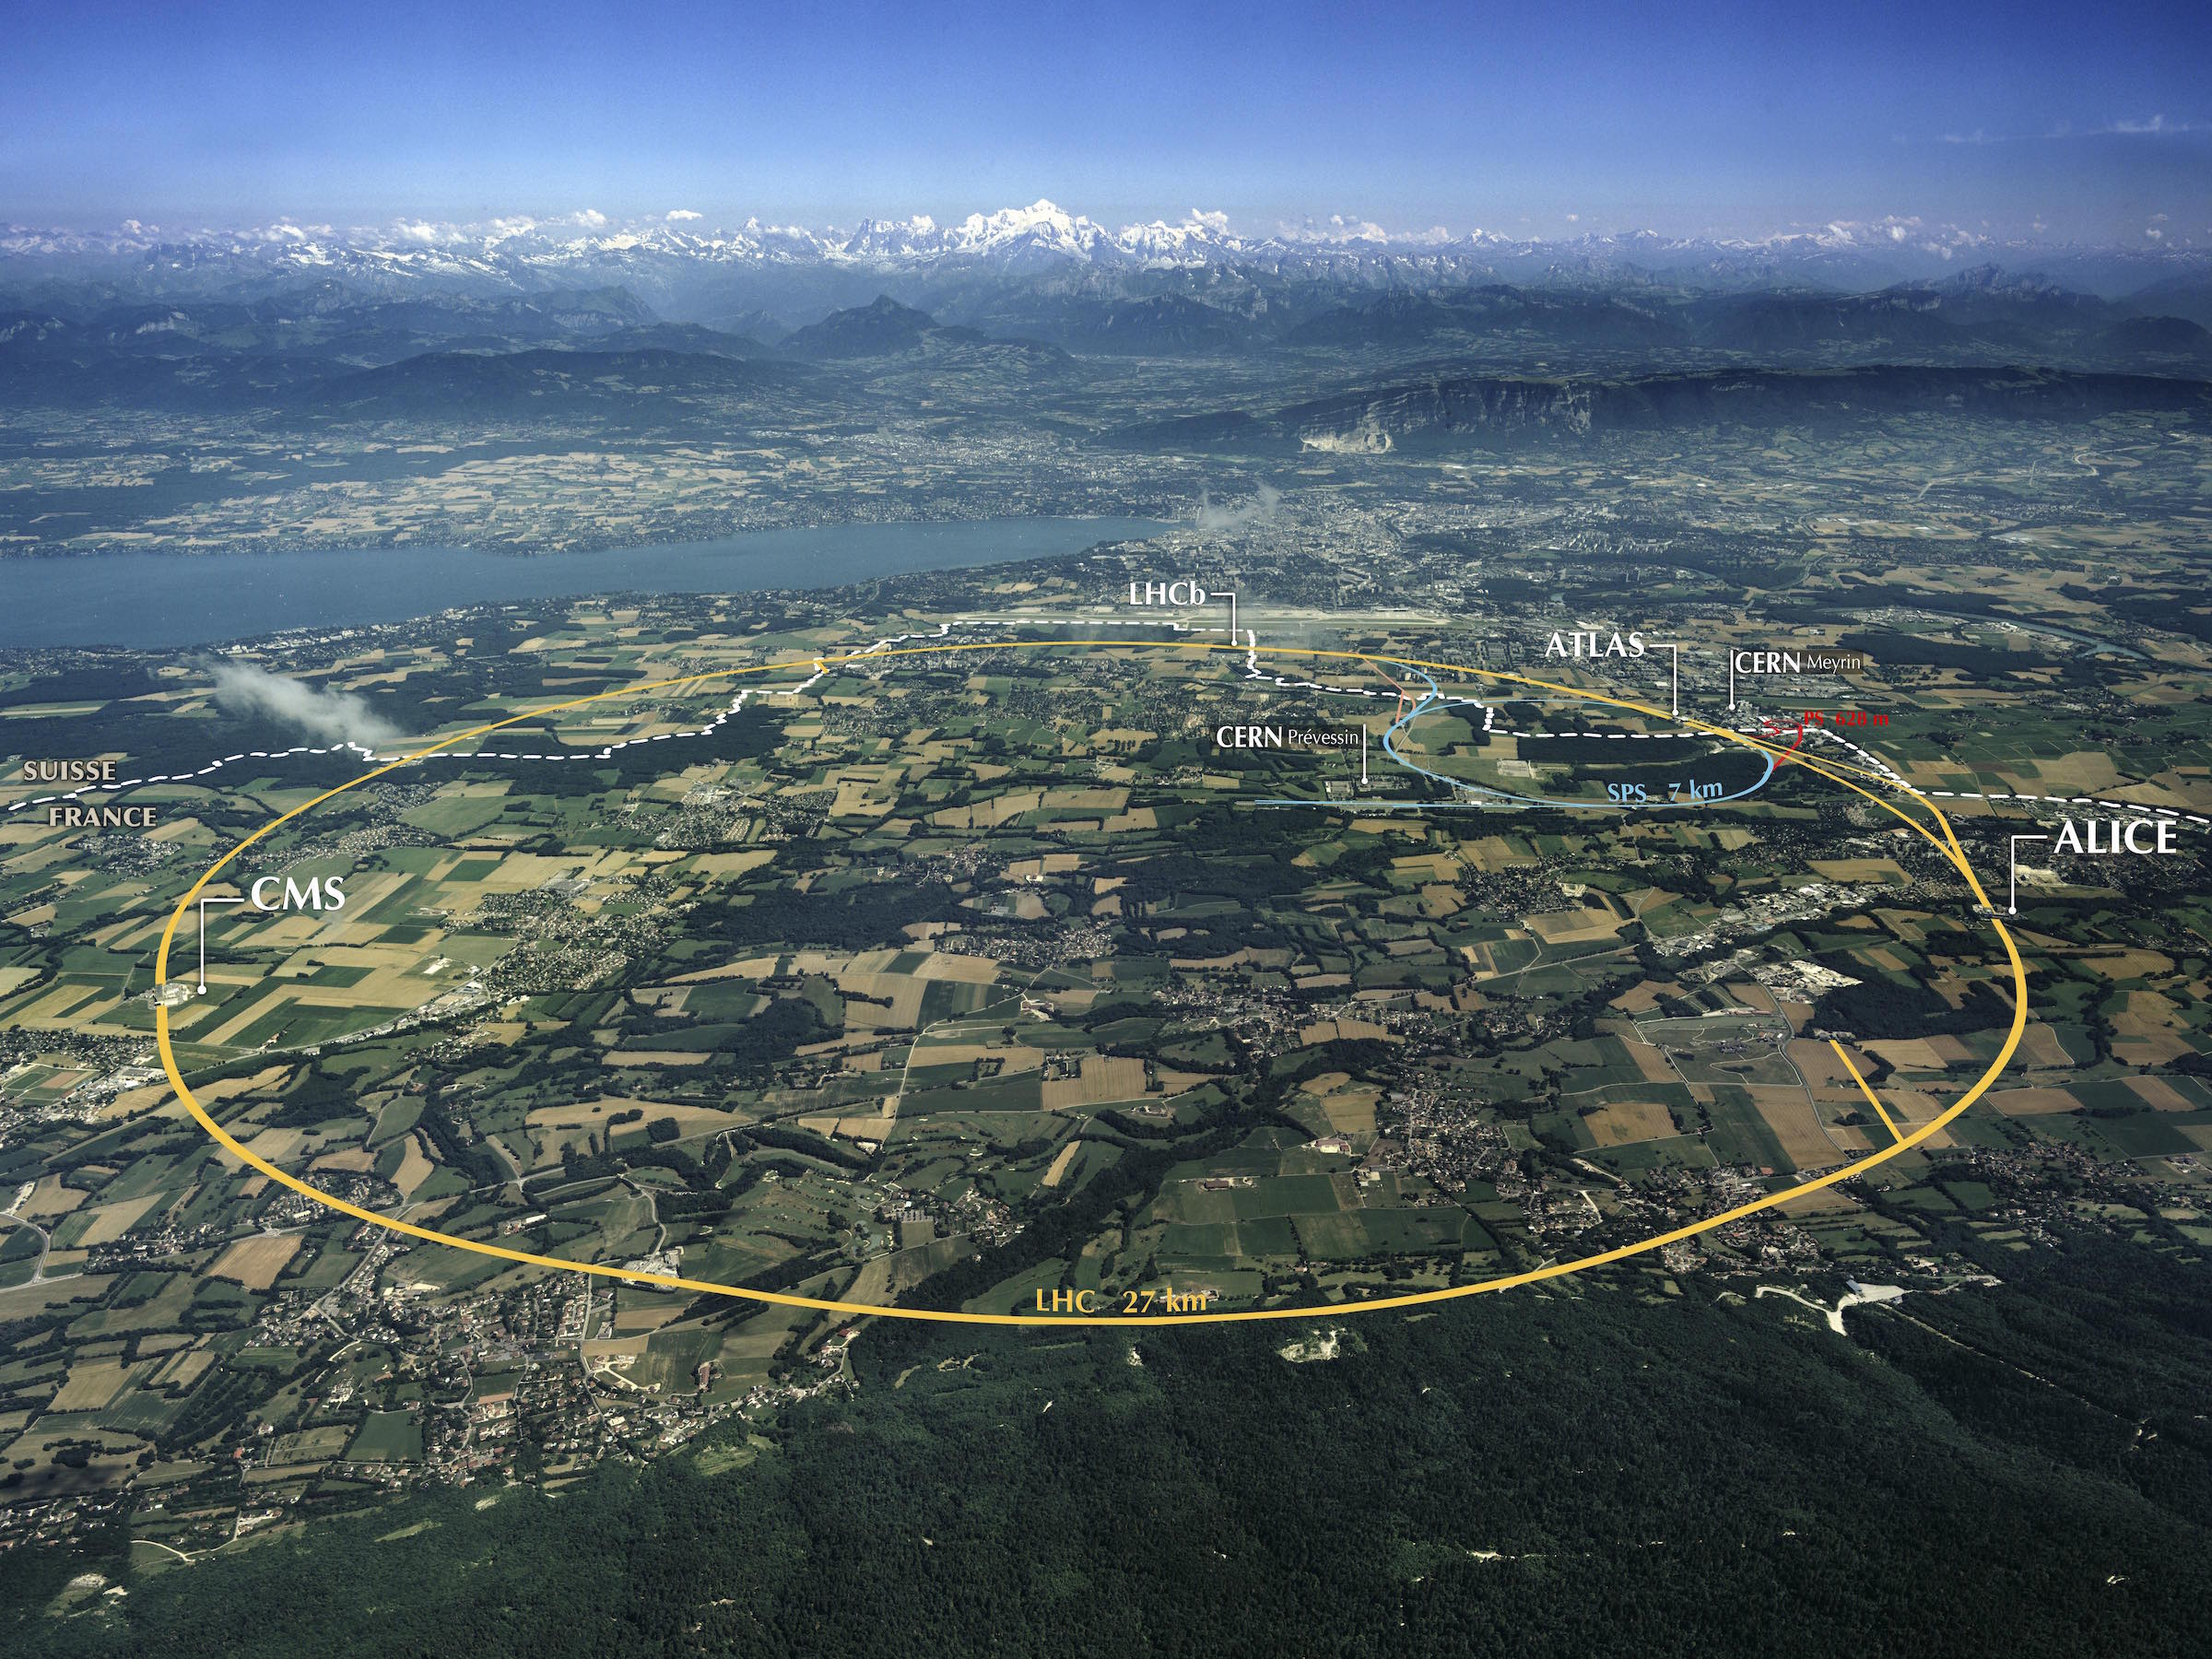
\includegraphics[width=0.8\linewidth]{Figures/LHC.jpg}
\caption{An aerial view of the LHC near Geneva, Switzerland~\cite{LHC_view}}
\label{fig:LHC}
\end{figure}

The process the LHC uses sounds simple when put into common terms. It accelerated protons to speeds very close to the speed of light and collides them at the center of a detector to see what comes out of these collisions. However actually accomplishing this is not simple at all. To start this process, electrons are stripped off from hydrogen gas, supplying the protons for the LHC. After this, the protons are put into a series of different accelerators, each designed to accelerate protons to higher and higher energies. The first accelerator is the Linac2 linear accelerator, which pushes the protons up to 50 MeV. Then they are sent to the Proton Synchrotron Booster which can push them to 1.4 GeV, after which the Proton Synchrotron ring accelerates the protons to 25 GeV. At this point protons are arranged into bunches such that a proton bunch passes by every 25~ns. This is the frequency at which protons collide in the LHC. Each bunch has about 100 billion protons in it. After sorted into these bunches, the protons are sent to the Super Proton Synchrotron where they achieve an energy of 450 GeV. Finally, the protons are fed into the LHC where they will be accelerated to their highest energy. An illustration of all of these accelerators is shown in figure~\ref{fig:acceleratorcomplex}.

\begin{figure}
\centering
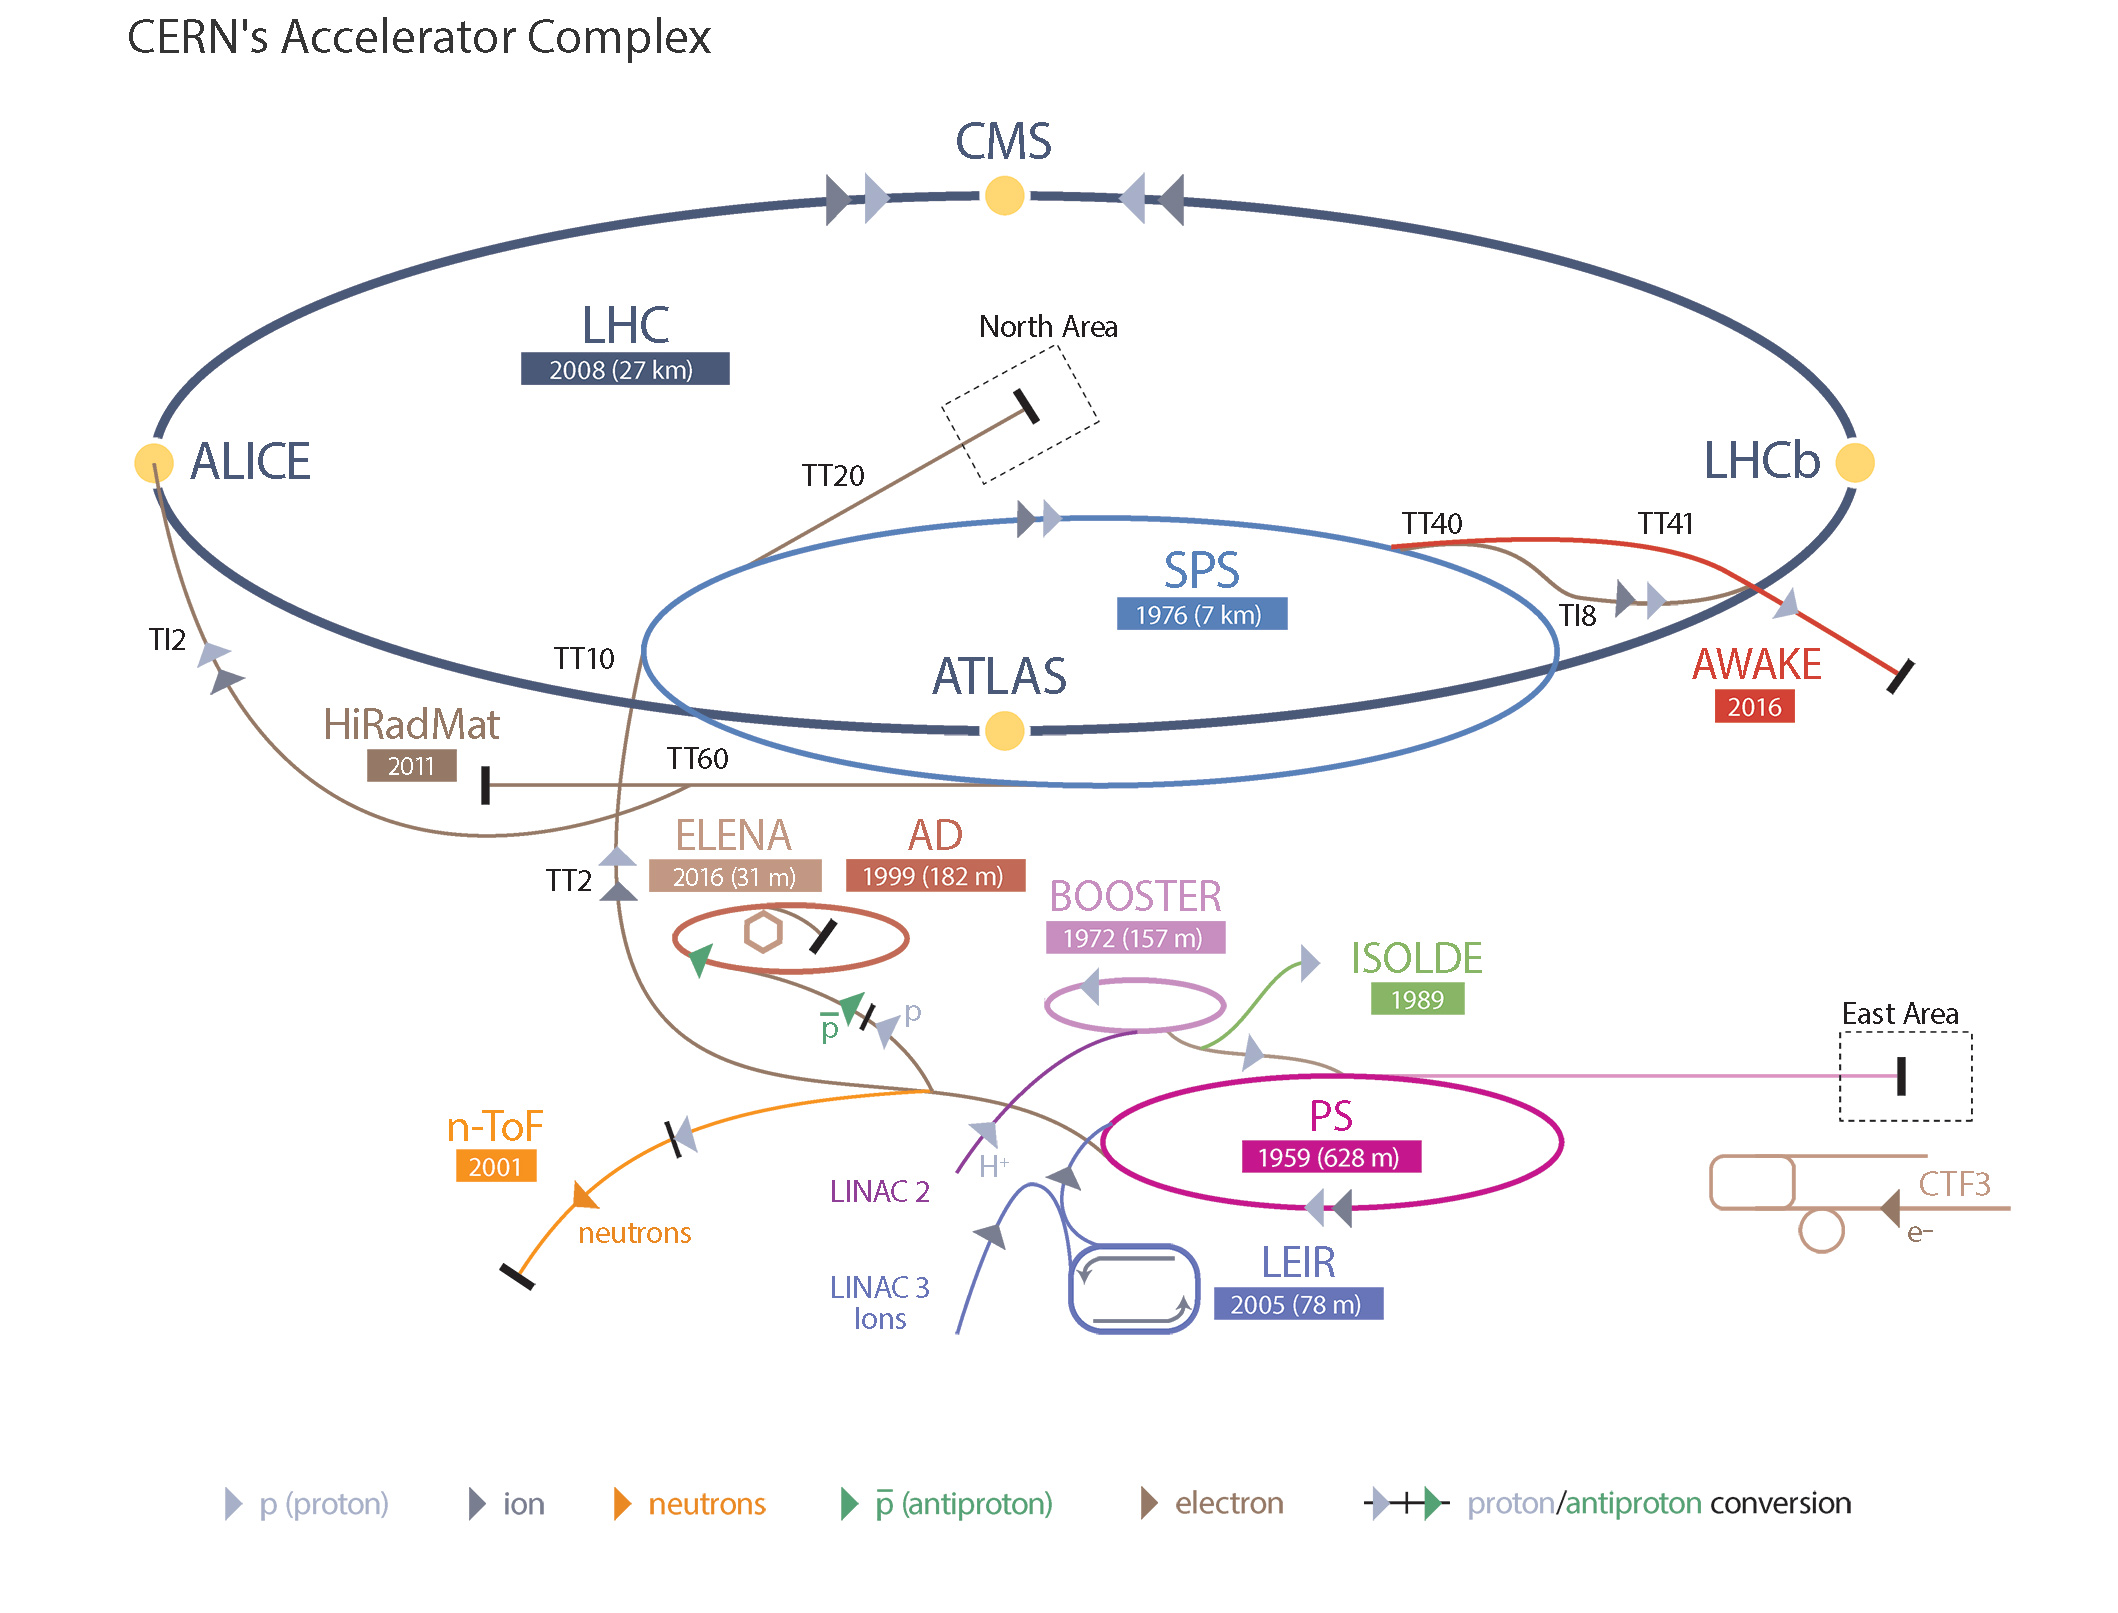
\includegraphics[width=0.8\linewidth]{Figures/acceleratorcomplex.jpg}
\caption{The chain of accelerators that feeds the protons into the LHC}
\label{fig:acceleratorcomplex}
\end{figure}

When the LHC has accelerated its particles to its peak energy it collides the particles in the middle of four different detectors. LHCb, ALICE, ATLAS, and CMS~\cite{CMS} are the names of the four detectors that were built to study collisions supplied by the LHC. The CMS detector is the one I worked on during my undergraduate career, and is discussed in detail below.

\section{The CMS Detector}
The CMS detector is designed to detect particles coming out of the proton-proton collisions supplied by the LHC. As many different types of particles come out of these collisions the CMS detector is split up into several different sub-detectors, each designed to measure different properties of different types of particles. Going from the closest to the collision point outward, first is the Silicon Tracker. The Silicon Tracker is capable of finely measuring the path of the charged particles that go through it. The CMS detector produces a 4 Tesla magnetic field throughout most of the detector. As charged particles move through the magnetic field, their path curves. The Silicon Tracker allows us to measure the curvature of their path and find their momentum. Next is the Electromagnetic Calorimeter which is mainly responsible for measuring the energy of photons and electrons that come out of the collision. Then there is the Hadron Calorimeter (HCAL) which is responsible for detecting hadrons, which are particles made up of quarks, such as protons neutrons and charged pions. The HCAL, along with the other sub-detectors, covers the collision point such that all paths out of the collision lead to the calorimeter. Since I did my work on the HCAL it is described in more detail in section~\ref{HCAL} Finally, there are the Muon Chambers. Unlike other particles the muon tends to just go through the calorimeters only losing a small portion of its energy. This means the muons will reach the last section of the detector mostly unperturbed. Since the muons are charges their path will be curved by the magnetic field so their momentum is measured by a process similar to that of the Silicon Tracker. An illustration of the of the different sub-detectors and the particles that will interact with them is shown in figure~\ref{fig:CMSlayout}.

Even with all of these sub-detector there are still particles not directly detected. Neutrinos for example tend to go through everything without interacting, and they do not appear in our detector's signals. Several of the particles on table~\ref{tab:particles} decay before ever reaching the detector. To find evidence of these particles we have to find indirect evidence of them. For example, the top quark nearly 100\% of the time decays into a bottom quark and a W boson. The W boson then either decays into a charged lepton neutrino pair or a light quark anti-quark pair. By finding evidence of these particles in close proximity we can deduce these came from a top quark.

\begin{figure}
\centering
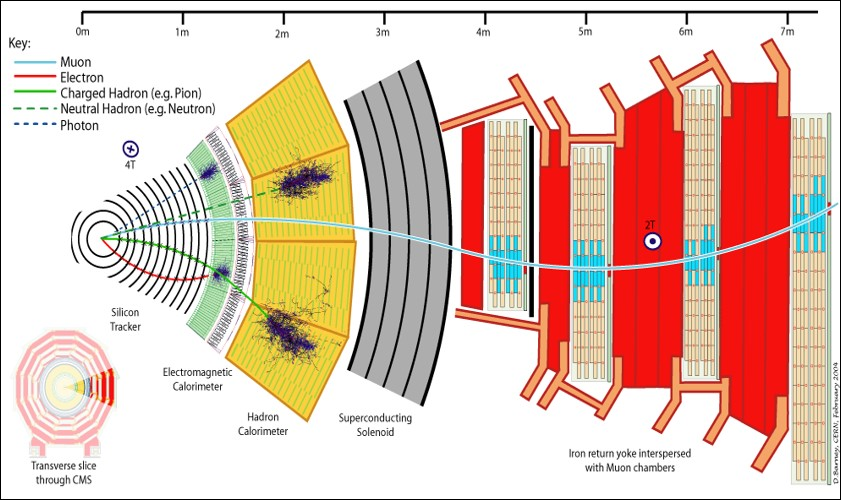
\includegraphics[width=\linewidth]{Figures/CMSlayout.jpg}
\caption{A slice of the CMS detector highlighting the different sub-detectors and showing different particles and where they are stopped~\cite{Davis}.}
\label{fig:CMSlayout}
\end{figure}

\subsection{Hadron Calorimeter} \label{HCAL}
One of the main jobs of the calorimeter is to measure the energy of the of the incident particle. To accomplish this, an absorber, made with brass in the HCAL, is placed in alternating layers with a scintillator tile. When a particle hits the nucleus of the absorber, they will produce a shower of secondary particles, which is called a hadronic shower. When these secondary particles hit the scintillator tile they will interact with the molecules in the tile exciting them. These molecules will return to their original energy state emitting a photon. This photon, which is usually blue, will travel through the tile into a wavelength shifting fiber around the edge of the tile, as shown in figure~\ref{fig:Tile}. The fiber will shift the photon into a green wavelength keeping it from exiting the fiber. After traveling through the fiber the photon will enter a light mixer. This device will collect the light from multiple fibers, mix them, and send them to the photo-detector, ensuring consistent and even distribution of the light on the next component. The original photo-detector for the HCAL was the hybrid photo-diodes (HPD)~\cite{HPD} but they are being replaced by silicon photomultipliers as apart of the upgrades on the CMS detector~\cite{HCALPhase1}. When the light is sent to the photo-detector it will output charge proportional to the number of incident photons. The shower of secondary particles will scatter throughout several scintillator tiles, and summing the output charge over all of the tiles will give a measurement of the energy of the incident particle. 
\begin{figure}
\centering
\includegraphics[width=0.6\linewidth]{Figures/Tile.png}
\caption{A scintillator tile with blue light and the wavelength shifting optical fiber around the edges and traveling out of the tile.}
\label{fig:Tile}
\end{figure}


There are three main section to the HCAL. There is the Hadron Barrel (HB)~\cite{HB}, which surrounds the beam-line like the edge of a cylinder, the Hadron Endcap (HE), which caps off the cylinder made by HB. These two parts make a cylinder which houses the beam-line going through the center of the caps and the collision point in the center. Lastly there is the Hadron Forward (HF) which is in a shape similar to the HE but is located much further away from the collision point~\cite{HF}. To describe the geometry of the detector we use a coordinate system related to spherical coordinates with the origin being the collision point and polar angle of 0 being along the beam-line. The azimuthal angle is denoted $\phi$ and the pseudo rapidity angle $\eta$ is related to the polar angle by $\eta = -\ln(\tan(\theta/2))$ which gives a value of 0 perpendicular to the beam-line and $\pm\infty$ along the beam-line. Usually these coordinates are arranged into discrete integer values denoted iphi and ieta, which are arranged such that a scintillator tile covers one ieta and one iphi as shown in figure~\ref{fig:Depth} but there are exception to this. For HB and HE there is also the segmentation in "depth" from the front face to the back end as shown in figure~\ref{fig:Depth} and each depth is denoted by an integer value. 


\begin{figure}
\centering
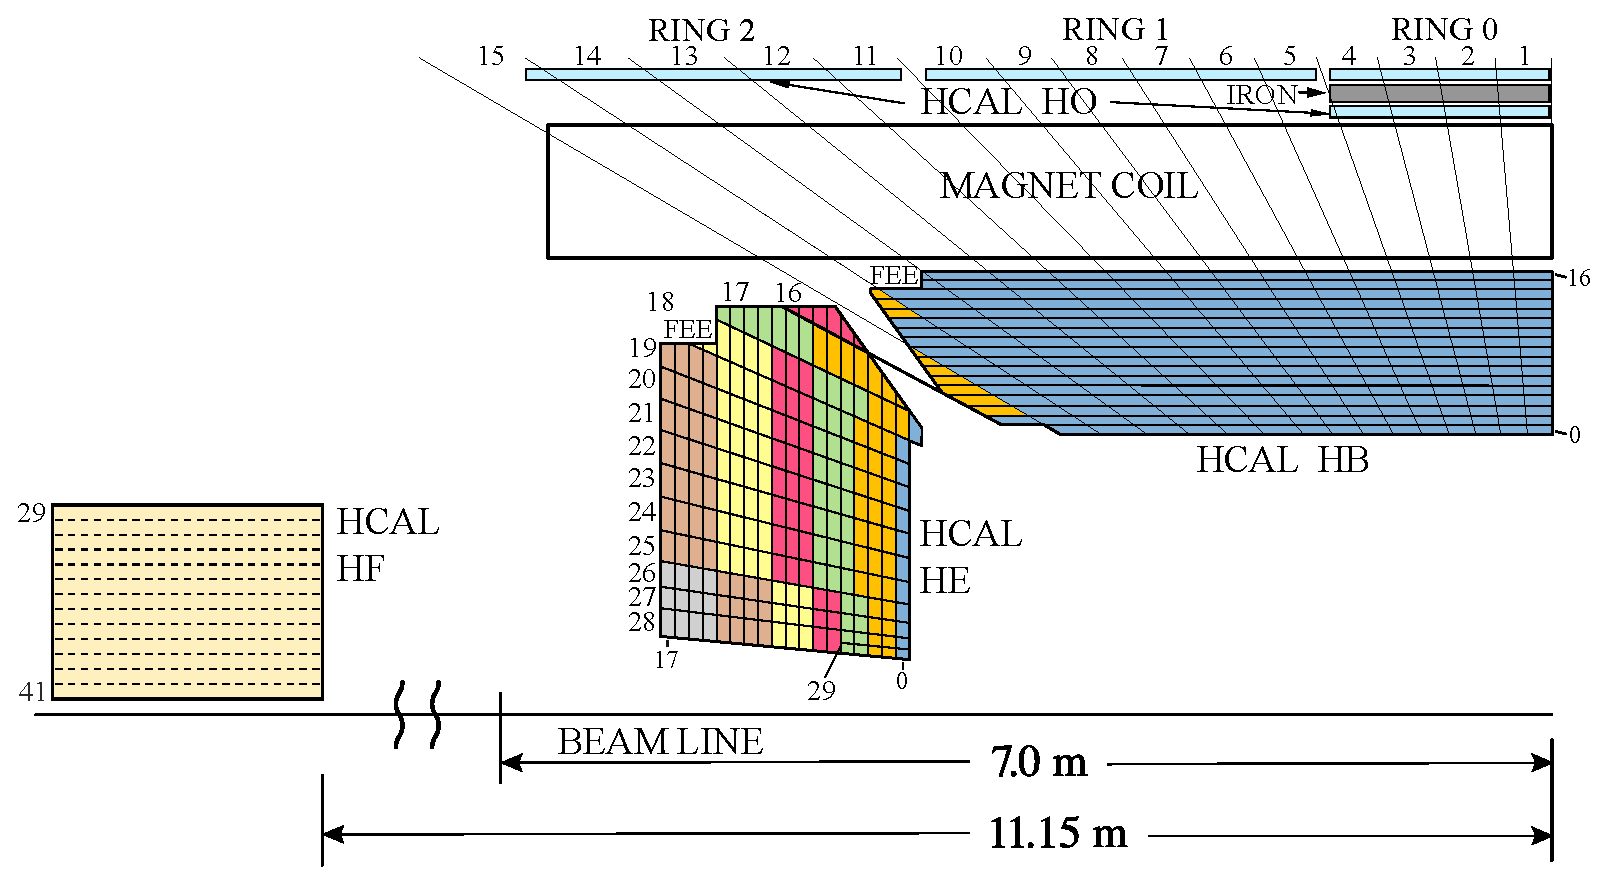
\includegraphics[width=\linewidth]{Figures/Depthsegmentation.pdf}
\caption{Layout of the HCAL showing a single iphi slice of HE, HB, and HF. Each box represents a scintillator tile}
\label{fig:Depth}
\end{figure}

\subsection{Silicon Photomultipliers}
The SiPM does its job of counting the photons from the scintillator by shining them on a pixel face. This is a circular array of really small pixels. A picture of the SiPM is in figure~\ref{fig:SiPM} showing several pixel faces. There are about 33,000 pixels on a 3.3 mm diameter pixel face. When an individual photon hits one of the pixels on the pixel face it causes a capacitor to fire off a particular amount of charge. The total output charge of the SiPM is the sum of all of the pixels output charge. Theoretically one just needs to sum the total amount of output charge of the SiPM and one can count the number of incident photons since each pixel will fire off a set amount of charge. Counting of the number of incident photons will give a measurement of the incident particles energy. There are some things that complicate the SiPMs readings. SiPMs are non-linear devices, meaning the total output charge of the SiPM does not necessarily increase linearly with the number of incident photons. In fact, experiments have shown that the number of incident photons vs. the SiPM output charge is more like a square root function rather than a straight line. At low incident photon count on the order of 1,000 photons the SiPM is very close to a linear device; however, as the incident number of photons increases the output charge does not increase at a steady rate. There are several factors that contribute to SiPM non-linearity but the two main ones are cross talk and saturation. Cross talk is when a pixel is activated by a photon there is a chance that this activated pixel could activate some of its neighboring pixels artificially increase the output charge of the SiPM. When the photon hits a pixel it excites an electron causing an electron cascade and charge to flow. This excited electron has a chance to emit an IR photon which could go in any direction. If it hits one of the neighboring pixels it could activate as if it were an incident photon. 

Saturation is when a pixel is hit in rapid succession by multiple photons. When a pixel is hit by a photon it discharges its capacitor which is the source of its output charge. After the pixel fires it needs some time on the order of 10 nanoseconds to recharge its capacitor. If the pixel is hit it simply fires off whatever charge it has in its capacitor at the time, which could be reduced from its normal charge. Given that the SiPM has about 33,000 pixels on its pixel face, when the number of incident is on the order of 1000 this effect is insignificant, but particles can produce much more photons where this effect can be much more significant. The non-linear properties of the SiPM makes it a bit harder to get accurate measurements, but there are ways to study them which will allow us to compensate for these affects.

\begin{figure}
\centering
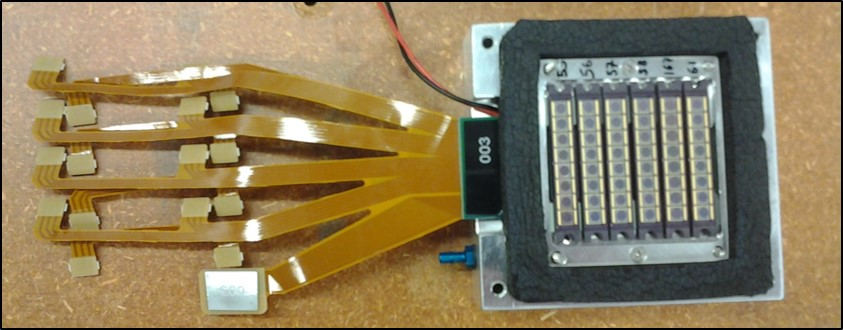
\includegraphics[width=\linewidth]{Figures/SiPM.jpg}
\caption{The silicon photomultiplier with several pixel faces.}
\label{fig:SiPM}
\end{figure}




